\chapter{Sprint 2 : Gestion des Tenants et Experts}

\section*{Introduction}

Ce chapitre présente la réalisation du \textbf{sprint 2} de TalentFlow, en lien avec
les user stories US03 et US04 du backlog produit (chapitre~2). Après validation du
compte entreprise au sprint~1, le recruteur (tenant) accède à son espace dédié :
tableau de bord, gestion multi-sociétés, configuration du profil et équipe d'experts RH.
Nous détaillons l'objectif du sprint, son backlog, l'analyse des cas d'utilisation
et les interfaces réalisées.

% ============================================================
\section{Objectif du Sprint}
% ============================================================

L'objectif principal de ce sprint est de déployer l'\textbf{espace recruteur} et la
\textbf{collaboration RH} au sein du modèle multi-tenant :

\begin{itemize}
    \item Mettre à disposition l'\textbf{espace recruteur} (\texttt{/recruiter/*}) :
    tableau de bord, navigation latérale et indicateurs d'activité.

    \item Permettre la \textbf{gestion multi-sociétés} : création et administration des
    entités \texttt{Entreprise} rattachées au \texttt{Tenant} via \texttt{TenantId}.

    \item Configurer le \textbf{profil tenant} (\texttt{TenantProfile}) : identité du
    recruteur, présence en ligne (site web, réseaux sociaux), stack technique et
    statut de recrutement.

    \item Gérer les \textbf{experts RH} : invitation par email, rattachement à une
    entreprise, consultation des candidatures et entretiens dans un espace expert dédié
    (\texttt{Expert}, rôle \texttt{Utilisateur.Expert}).
\end{itemize}

% ============================================================
\section{Analyse du Sprint 2}
% ============================================================

\subsection{Sprint Backlog}

Le tableau~\ref{tab:backlog_s2} présente les user stories réalisées durant ce sprint.

\begin{table}[h]
\centering
\renewcommand{\arraystretch}{1.4}
\begin{tabular}{|c|p{8.5cm}|c|}
\hline
\textbf{ID} & \textbf{User Story} & \textbf{Priorité} \\
\hline
US03 & En tant qu'administrateur, je veux valider et configurer les tenants pour assurer
leur onboarding (prérequis : compte \texttt{Approved}). & Haute \\
\hline
US04 & En tant que tenant, je veux gérer les experts (\texttt{Expert}) et les entreprises
(\texttt{Entreprise}) de mon espace. & Haute \\
\hline
US04a & En tant que tenant, je veux consulter un tableau de bord récapitulatif de mon
activité de recrutement. & Haute \\
\hline
US04b & En tant que tenant, je veux configurer mon profil et l'environnement de mon
société (\texttt{TenantProfile}). & Haute \\
\hline
US04c & En tant que tenant, je veux inviter un expert par email et le rattacher à une
entreprise. & Haute \\
\hline
US04d & En tant qu'expert, je veux accéder à mon espace (dashboard, candidatures,
entretiens) après invitation. & Haute \\
\hline
\end{tabular}
\caption{Sprint Backlog du Sprint 2}
\label{tab:backlog_s2}
\end{table}

\subsection{Diagramme de Cas d'Utilisation — Sprint 2}

\begin{figure}[ht]
    \centering
    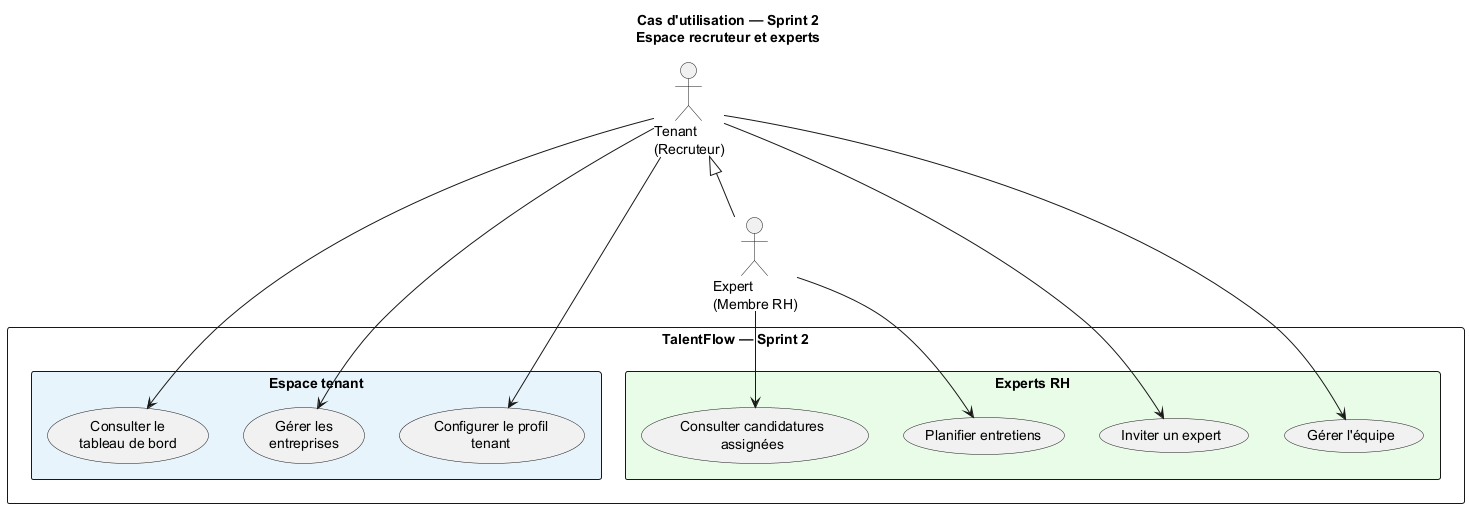
\includegraphics[width=0.95\textwidth]{images/usecase_sprint2.png}
    \caption{Diagramme de cas d'utilisation du Sprint 2}
    \label{fig:uc_sprint2}
\end{figure}

\subsubsection{Description Textuelle des Cas d'Utilisation}

\textbf{Cas d'utilisation : Gérer les entreprises partenaires}

\begin{itemize}
    \item \textbf{Acteur principal :} Tenant (recruteur)
    \item \textbf{Scénario nominal :} le recruteur accède à \textit{Companies}, consulte
    la liste des sociétés (\texttt{Entreprise}), ajoute une entreprise (nom, secteur, RNE,
    logo) ou modifie une fiche existante.
    \item \textbf{Postcondition :} l'entreprise est rattachée au \texttt{TenantId} du
    recruteur connecté.
\end{itemize}

\textbf{Cas d'utilisation : Inviter un expert RH}

\begin{itemize}
    \item \textbf{Acteur principal :} Tenant
    \item \textbf{Scénario nominal :}
    \begin{enumerate}
        \item Le recruteur ouvre \textit{Team Management} et clique sur \textit{Add Expert}.
        \item Il renseigne prénom, nom, email, entreprise cible et poste.
        \item Le système crée \texttt{Expert} et \texttt{Utilisateur} (rôle \texttt{Expert}),
        puis envoie un courriel avec mot de passe temporaire.
    \end{enumerate}
    \item \textbf{Postcondition :} l'expert se connecte et accède à \texttt{/expert/dashboard}.
\end{itemize}

% ============================================================
\section{Réalisation}
% ============================================================

\subsection{Tableau de Bord Recruteur}

Après connexion avec un compte tenant \texttt{Approved}, le recruteur accède au
tableau de bord (\texttt{TenantDashboard.vue}, route \texttt{/recruiter/dashboard}).
La page affiche des indicateurs (offres publiées, candidatures du mois, recrutements
réussis), un tableau des offres récentes et un aperçu des dernières candidatures.
Le bouton \textit{New job offer} renvoie vers le module offres (chapitre~5).

\begin{figure}[ht]
    \centering
    \includegraphics[width=\textwidth]{images/tenant_dashboard.jpg}
    \caption{Tableau de bord de l'espace recruteur}
    \label{fig:tenant_dashboard}
\end{figure}

\subsection{Gestion des Entreprises Partenaires}

La page \textit{Companies} (\texttt{Companys.vue}) centralise les sociétés du tenant.
Des cartes récapitulent le nombre total d'entreprises, le statut du compte
(\textit{Approved}) et le nombre d'offres associées. Chaque carte affiche le logo,
le secteur, le nombre d'experts et d'offres, ainsi que les actions d'édition et
de suppression. Le bouton \textit{Add company} ouvre une modale de création.

\begin{figure}[ht]
    \centering
    \includegraphics[width=\textwidth]{images/companys_list.jpg}
    \caption{Gestion des entreprises partenaires (multi-sociétés)}
    \label{fig:companys_list}
\end{figure}

\subsection{Configuration du Profil Tenant}

L'écran \textit{Company Owner's Profile} (\texttt{TenantProfile.vue},
\texttt{/recruiter/settings}) permet de configurer l'environnement du recruteur :
logo de la société, complétude du profil, informations du compte (nom, email, poste,
téléphone), présence en ligne (site web, LinkedIn, Twitter) et changement de mot de passe.
Les données sont persistées dans \texttt{TenantProfile} et liées au \texttt{TenantId}.

\begin{figure}[ht]
    \centering
    \includegraphics[width=\textwidth]{images/tenant_profile.jpg}
    \caption{Configuration du profil tenant et du recruteur}
    \label{fig:tenant_profile}
\end{figure}

\subsection{Gestion de l'Équipe — Experts RH}

La page \textit{Team Management} (\texttt{TeamManagement.vue}) liste les experts
du tenant avec recherche et filtre par entreprise. Des statistiques indiquent le nombre
de membres, de sociétés, d'assignations et la force du réseau. Pour chaque expert,
le recruteur peut modifier la fiche, assigner une offre (détail au chapitre~5) ou
supprimer le membre.

\begin{figure}[ht]
    \centering
    \includegraphics[width=\textwidth]{images/team_management.jpg}
    \caption{Gestion de l'équipe d'experts RH}
    \label{fig:team_management}
\end{figure}

\subsection{Invitation d'un Expert}

La modale \textit{Add New Expert} collecte le prénom, le nom, l'email, l'entreprise
(\texttt{CompanyId}) et le poste. À la validation, l'API \texttt{POST /api/expert/invite}
crée l'expert et déclenche l'envoi d'un courriel d'invitation (service email Brevo).

\begin{figure}[ht]
    \centering
    \includegraphics[width=0.75\textwidth]{images/team_invite_expert.jpg}
    \caption{Invitation d'un nouvel expert RH}
    \label{fig:team_invite_expert}
\end{figure}

\subsection{Courriel d'Invitation Expert}

Le message automatique confirme l'invitation à rejoindre l'entreprise cible sur
TalentFlow, décrit les missions de l'expert (évaluation des candidatures,
entretiens IA, collaboration RH) et fournit les identifiants de première connexion
(email et mot de passe temporaire avec date d'expiration).

\begin{figure}[ht]
    \centering
    \includegraphics[width=0.85\textwidth]{images/expert_invitation_email.jpg}
    \caption{Courriel d'invitation envoyé à l'expert}
    \label{fig:expert_email}
\end{figure}

\subsection{Espace Expert}

Une fois connecté, l'expert accède à un espace dédié (\textit{Expert Plan}) avec
un tableau de bord (offres assignées, pipeline candidats), la liste des candidatures,
le calendrier des entretiens et les paramètres du compte.

\begin{figure}[ht]
    \centering
    \includegraphics[width=\textwidth]{images/expert_dashboard.jpg}
    \caption{Tableau de bord de l'espace expert}
    \label{fig:expert_dashboard}
\end{figure}

\begin{figure}[ht]
    \centering
    \includegraphics[width=\textwidth]{images/expert_applications.jpg}
    \caption{Liste des candidatures vues par l'expert}
    \label{fig:expert_applications}
\end{figure}

\begin{figure}[ht]
    \centering
    \includegraphics[width=\textwidth]{images/expert_interviews.jpg}
    \caption{Calendrier des entretiens — espace expert}
    \label{fig:expert_interviews}
\end{figure}

\section*{Conclusion}

Le sprint 2 a livré l'espace recruteur opérationnel de TalentFlow. Le tenant gère
plusieurs \texttt{Entreprise}, configure son \texttt{TenantProfile} et constitue une
équipe d'\texttt{Expert} invités par email. L'espace expert permet de suivre les
candidatures et les entretiens sur les offres assignées. L'isolation par
\texttt{TenantId} garantit que chaque recruteur n'accède qu'à ses sociétés et à son
équipe. Le chapitre suivant présente le sprint~3 : création, personnalisation,
publication des offres d'emploi et diffusion par lien public tokenisé.
